% ============================================================
% PRM393 - Section 6: UI/UX, Navigation & Routing (Bilingual)
% ============================================================
\section{\bi{Thiết kế giao diện và hệ thống điều hướng}{UI/UX Design, Navigation \& Screen Hierarchy}}
\label{sec:ui}

\bi{
OmniCast Mobile định hình phong cách thiết kế theo chủ đề điện ảnh cao cấp
(\textbf{Cinema Dark Theme}), lấy tông đen tuyền (\texttt{\#0F172A}) và xanh
ngọc (\texttt{\#0E7490}) làm gam màu chủ đạo. Ngôn ngữ thiết kế này vừa tối
ưu hóa khả năng hiển thị nội dung video, vừa giúp tiết kiệm pin đáng kể trên
các màn hình công nghệ OLED/AMOLED.
}{
OmniCast Mobile embraces an elevated \textbf{Cinema Dark Theme}, anchoring its
visual palette around midnight slate (\texttt{\#0F172A}) and luminous cyan
(\texttt{\#0E7490}). This aesthetic highlights video and graphical media
while yielding significant power savings on modern OLED/AMOLED smartphone
displays.
}

\begin{figure}[t]
\centering
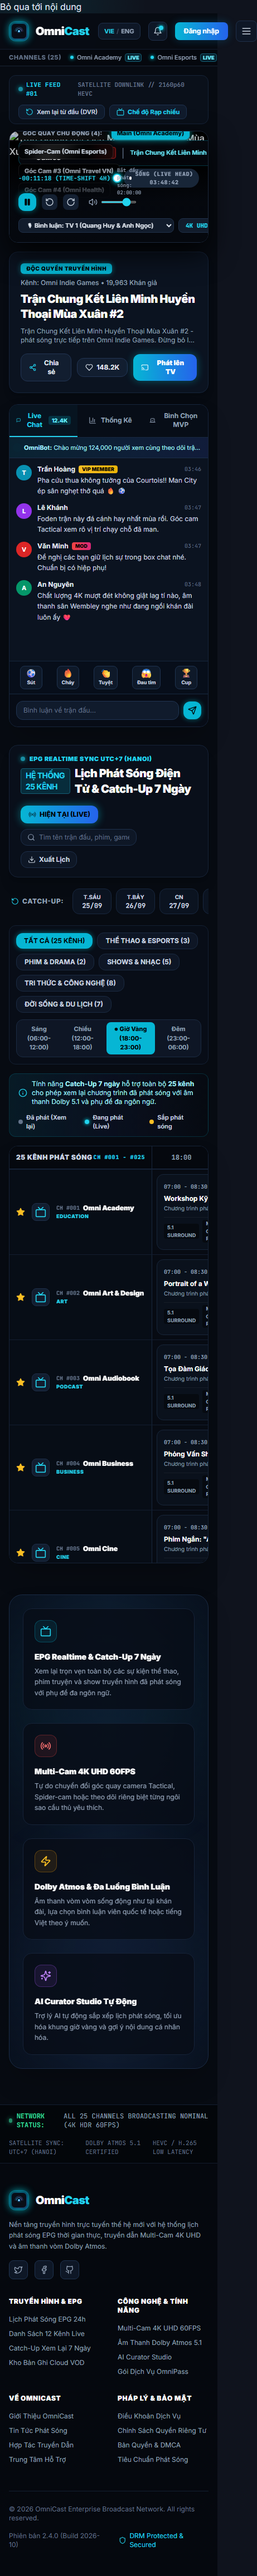
\includegraphics[width=0.6\columnwidth,height=6.5cm,keepaspectratio]{../figures/01_mobile_home.png}
\caption{\bi{Giao diện trang chủ OmniCast Mobile: carousel sự kiện nổi bật,
thanh chuyển kênh theo thể loại và các chương trình sắp phát sóng.}{The
OmniCast Mobile home view: featured broadcast carousel, category selector,
and upcoming electronic programme guide.}}
\label{fig:mob_home}
\end{figure}

\subsection{\bi{Hệ thống điều hướng khai báo với GoRouter}{Declarative Routing with GoRouter}}

\bi{
Toàn bộ luồng chuyển màn hình được điều khiển bởi gói \texttt{go\_router}
thông qua mô hình khai báo tập trung trong \texttt{app\_router.dart}. Mô hình
này mang lại ba ưu thế vượt trội:
}{
The client's comprehensive routing topology is orchestrated via
\texttt{go\_router} declared centrally in \texttt{app\_router.dart}. This
architecture unlocks three critical capabilities:
}

\begin{enumerate}[leftmargin=*,itemsep=2pt]
  \item \textbf{\bi{Bảo vệ tuyến đường theo phiên (Auth Guards):}{Auth-Guarded Redirection:}}
  \bi{Khi người dùng truy cập các màn hình cá nhân hóa như \texttt{/watchlist},
  \texttt{/studio} hoặc \texttt{/profile}, bộ định tuyến sẽ tự động kiểm tra
  trạng thái \texttt{AuthBloc}. Nếu chưa đăng nhập, người dùng sẽ được chuyển
  hướng an toàn về màn hình \texttt{/login} kèm tham số trả về (return URI).}{%
  Attempting to enter authenticated zones such as \texttt{/watchlist},
  \texttt{/studio}, or \texttt{/profile} triggers automatic redirection checks
  against \texttt{AuthBloc}. Unauthenticated sessions redirect to
  \texttt{/login} with preserved return query parameters.}

  \item \textbf{\bi{Hỗ trợ liên kết sâu (Deep Linking):}{Deep-Linking Support:}}
  \bi{Hỗ trợ phân giải các đường dẫn như \texttt{omnicast://channels/:id} hoặc
  \texttt{omnicast://events/:id}, cho phép mở chính xác màn hình chi tiết sự
  kiện từ các thông báo đẩy hoặc liên kết chia sẻ mạng xã hội.}{%
  Natively maps external URIs such as \texttt{omnicast://channels/:id} or
  \texttt{omnicast://events/:id}, routing users directly to destination views
  from push alerts or shared links.}

  \item \textbf{\bi{Điều hướng nhánh giữ trạng thái (StatefulShellRoute):}{StatefulShellRoute Bottom Navigation:}}
  \bi{Thanh điều hướng đáy (BottomNavigationBar) với 5 mục (Trang chủ, Kênh,
  Lịch phát EPG, Danh sách xem, Tài khoản) duy trì trạng thái cuộn và dữ liệu
  của từng tab riêng biệt, không làm tải lại dữ liệu khi người dùng chuyển
  đổi qua lại giữa các tab.}{%
  A 5-destination bottom navigation bar (Home, Channels, EPG, Watchlist,
  Account) preserves view hierarchies and scroll offsets across tab switches
  without re-fetching data.}
\end{enumerate}

\subsection{\bi{Phân nhóm 31 màn hình ứng dụng}{Hierarchy of the 31 Application Screens}}

\bi{
Hệ thống 31 màn hình được phân loại thành 5 khu vực chức năng rõ ràng:
}{
The 31 screens are partitioned across 5 functional operational domains:
}

\begin{itemize}[leftmargin=*,itemsep=2pt]
  \item \textbf{\bi{Xác thực \& Nhập môn (4 màn hình):}{Authentication \& Onboarding:}}
  \texttt{SplashScreen}, \texttt{OnboardingScreen}, \texttt{LoginScreen},
  \texttt{RegisterScreen}.
  \item \textbf{\bi{Khám phá nội dung (8 màn hình):}{Content Discovery:}}
  \texttt{HomeScreen}, \texttt{ChannelsScreen}, \texttt{ChannelDetailScreen},
  \texttt{EpgScreen}, \texttt{ProgramsScreen}, \texttt{ProgramDetailScreen},
  \texttt{RecordingsScreen}, \texttt{SearchScreen}.
  \item \textbf{\bi{Phát trực tiếp \& Tương tác (5 màn hình):}{Live \& Interactive:}}
  \texttt{LiveScreen}, \texttt{LivePlayerScreen}, \texttt{LiveChatSheet},
  \texttt{LiveDonationModal}, \texttt{ReactionOverlay}.
  \item \textbf{\bi{Phòng thu Studio \& Sáng tạo (6 màn hình):}{Creator Studio:}}
  \texttt{StudioDashboardScreen}, \texttt{LiveStudioScreen},
  \texttt{AiCuratorScreen}, \texttt{ProgramEditorScreen},
  \texttt{ScheduleManagerScreen}, \texttt{StreamConfigScreen}.
  \item \textbf{\bi{Cá nhân hóa \& Cài đặt (8 màn hình):}{Personalization \& Settings:}}
  \texttt{WatchlistScreen}, \texttt{WatchHistoryScreen},
  \texttt{NotificationsScreen}, \texttt{ProfileScreen},
  \texttt{EditProfileScreen}, \texttt{SettingsScreen},
  \texttt{AboutScreen}, \texttt{HelpFaqScreen}.
\end{itemize}

\begin{figure}[t]
\centering
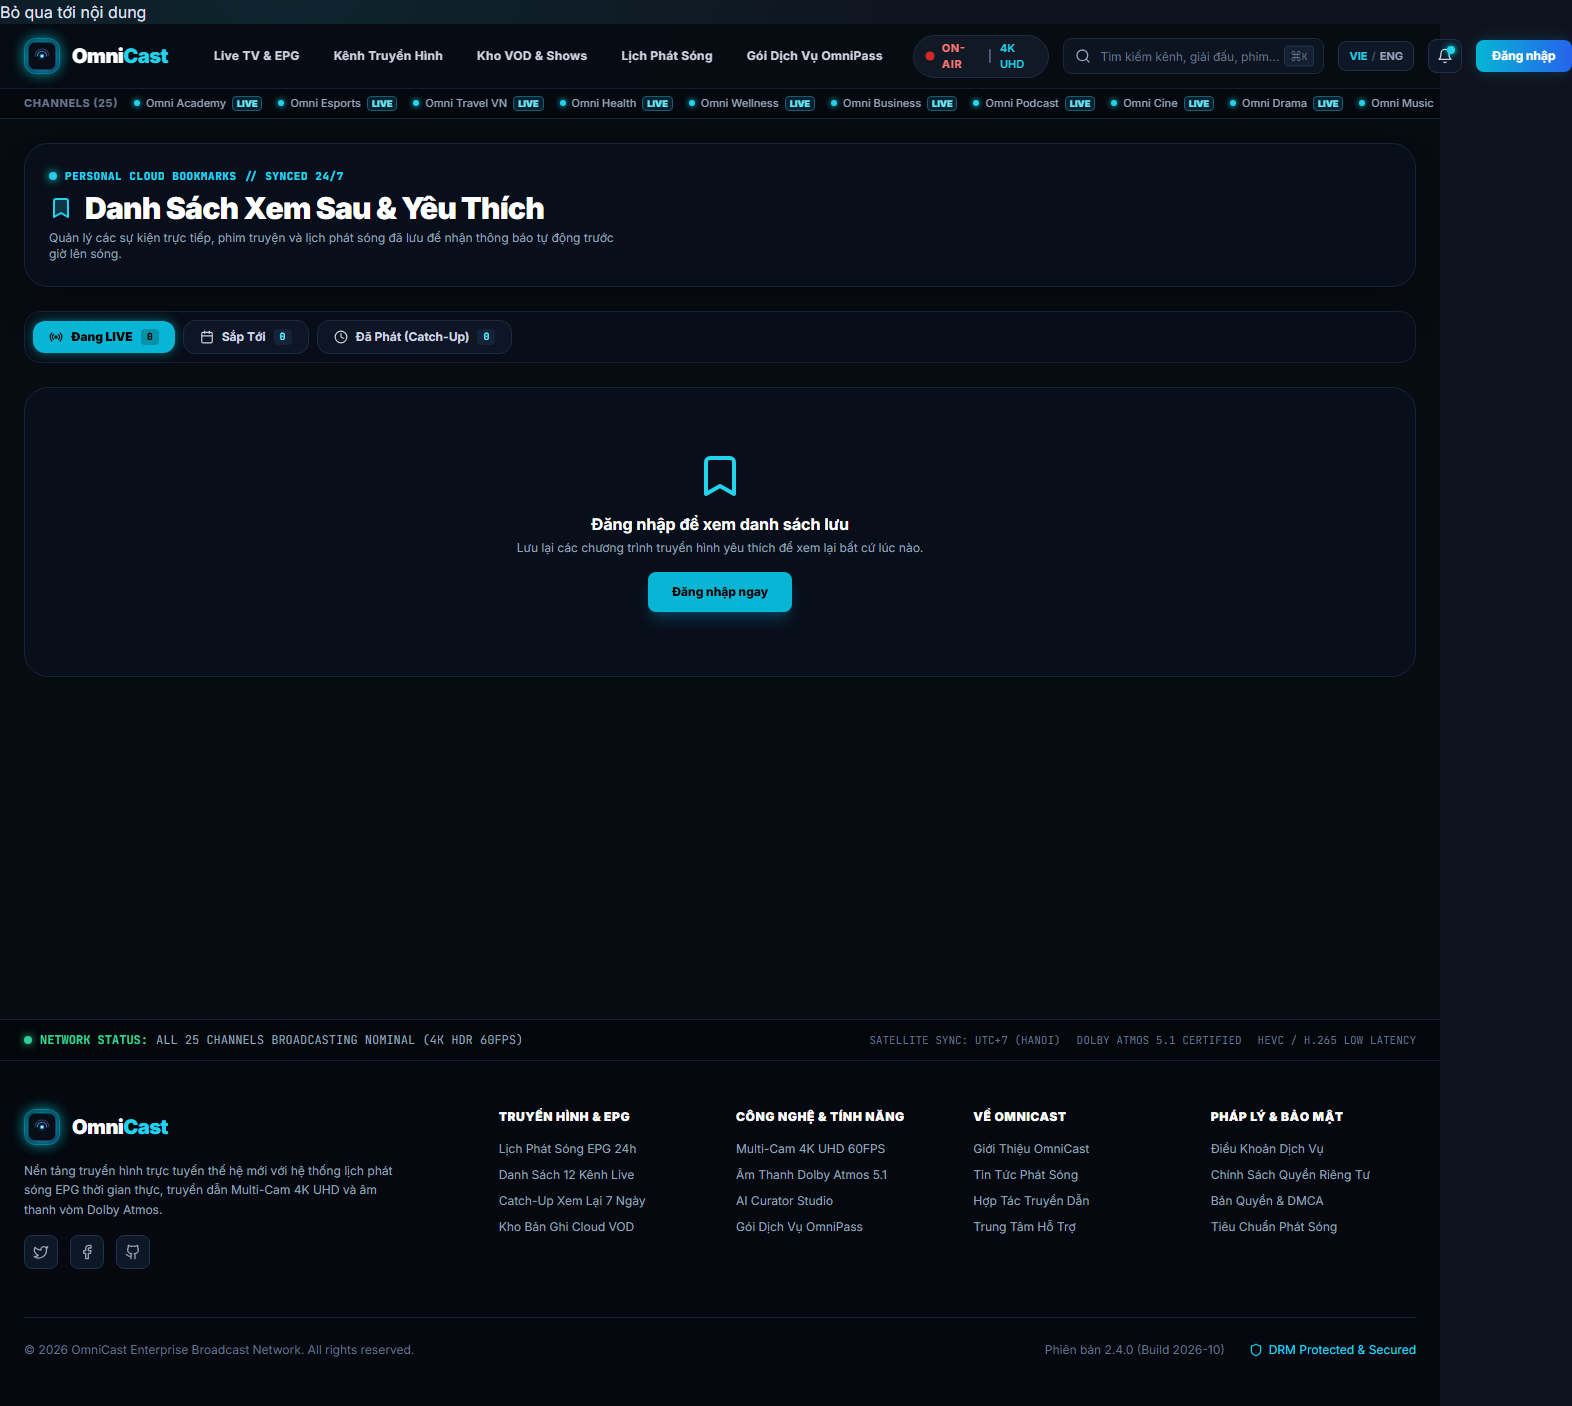
\includegraphics[width=0.48\columnwidth,height=5.2cm,keepaspectratio]{../figures/02_watchlist_screen.png}
\hfill
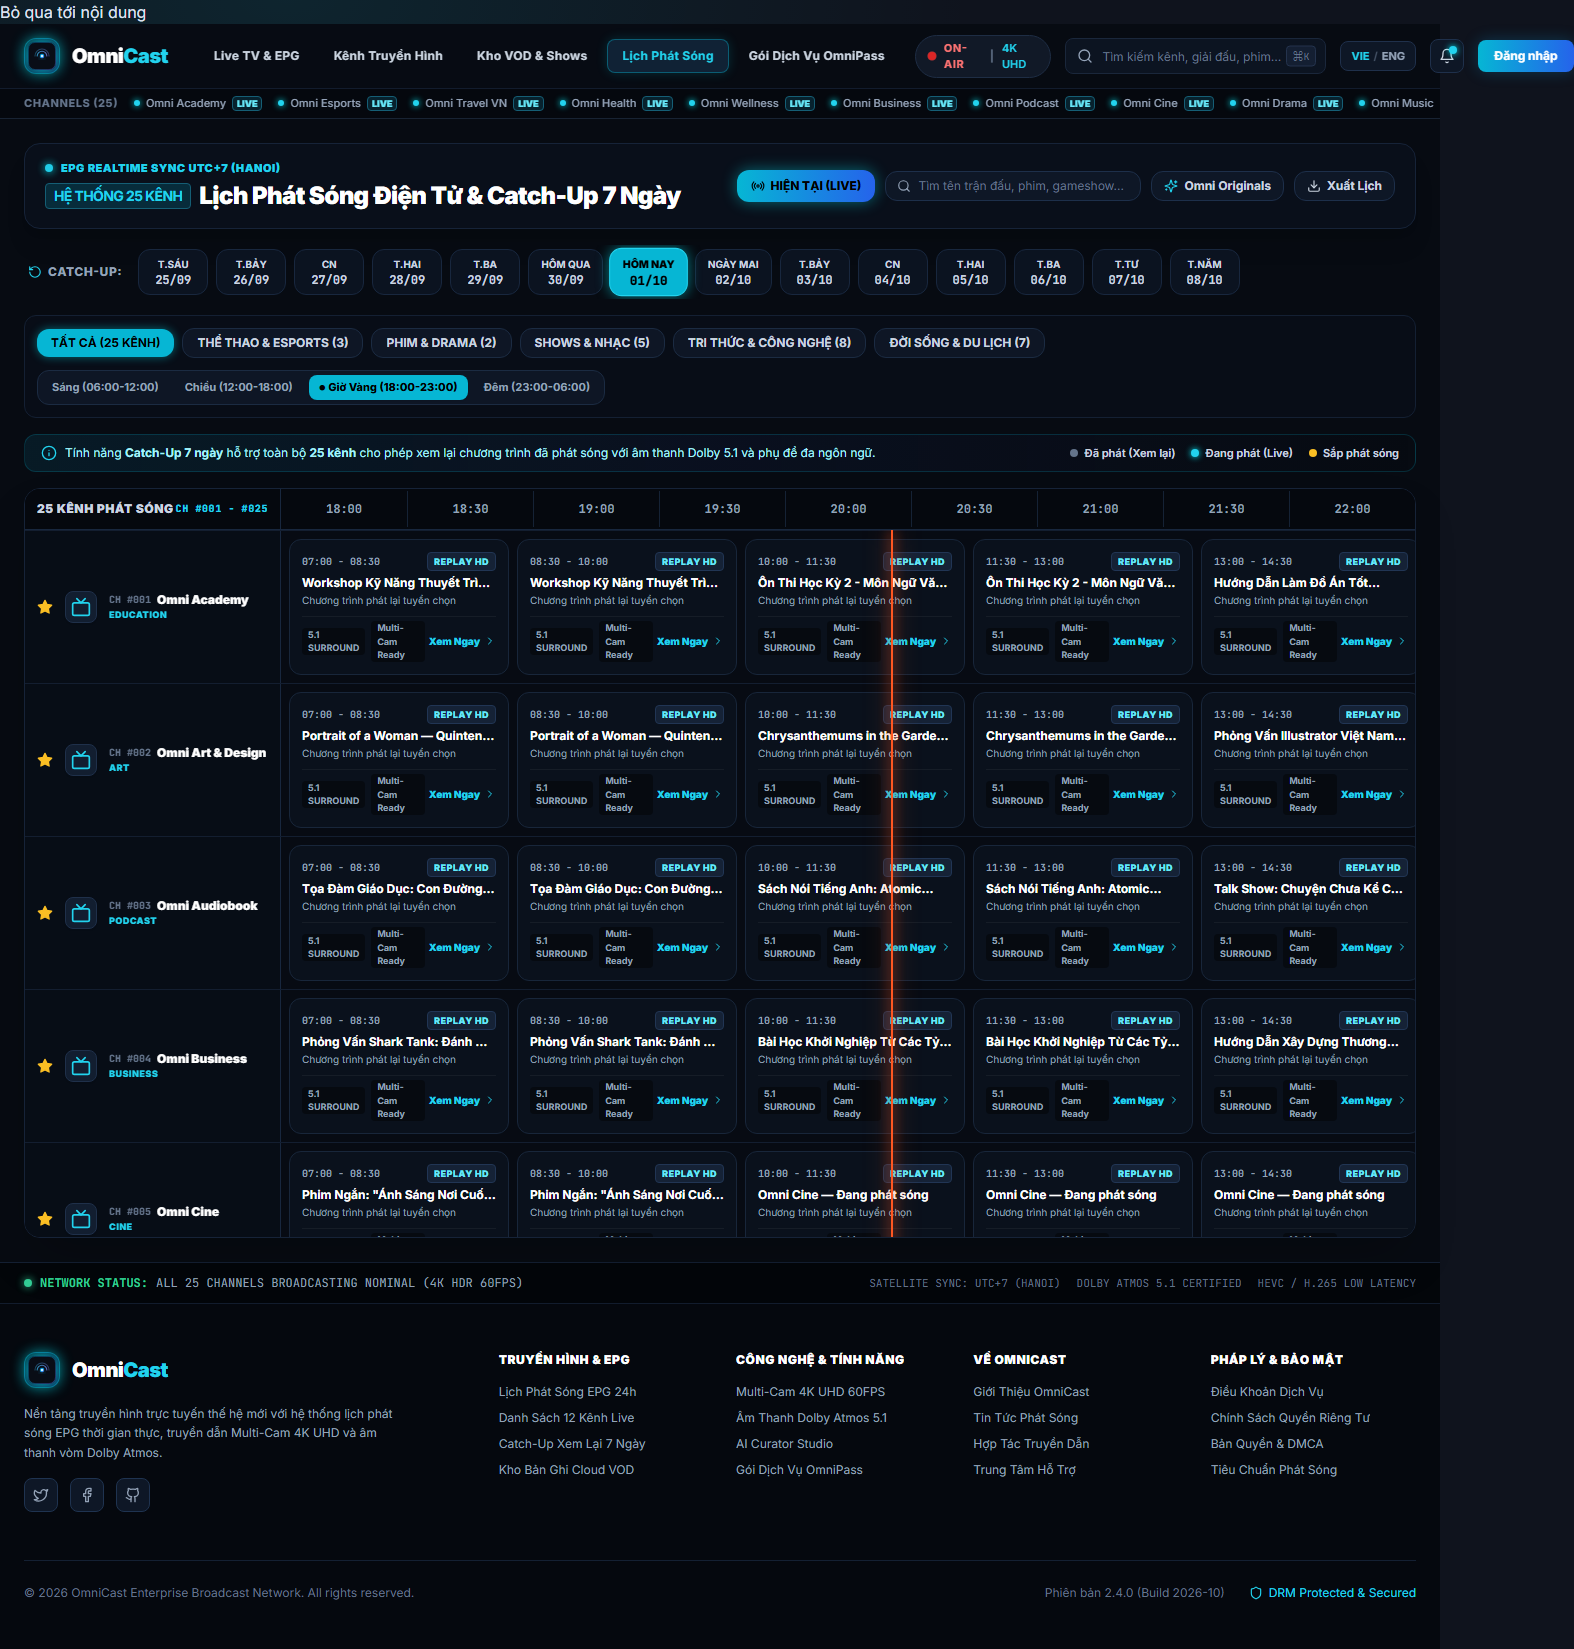
\includegraphics[width=0.48\columnwidth,height=5.2cm,keepaspectratio]{../figures/03_epg_screen.png}
\caption{\bi{Giao diện Danh sách theo dõi hỗ trợ lọc ngoại tuyến (trái) và
Lưới phát sóng điện tử EPG theo dòng thời gian 24/7 (phải).}{Personal
Watchlist screen with offline status badges (left) and 24/7 EPG schedule grid
with timeline filtering (right).}}
\label{fig:mob_subscreens}
\end{figure}
